% Rollout qualitative examples (ICLR layout).
% PDFs: pointmaze_dinowm_unsuccessful_iclr.pdf, pointmaze_dinobisim_successful_iclr.pdf,
%       pusht_dinowm_unsuccessful_iclr.pdf, pusht_dinobisim_successful_iclr.pdf
%
% Requires: \usepackage{graphicx,subcaption} (or subfig)

% ---------------------------------------------------------------------------
% Option A — four panels in one figure* (recommended for appendix / full width)
% ---------------------------------------------------------------------------
\begin{figure*}[t]
  \centering
  \begin{subfigure}[t]{\textwidth}
    \centering
    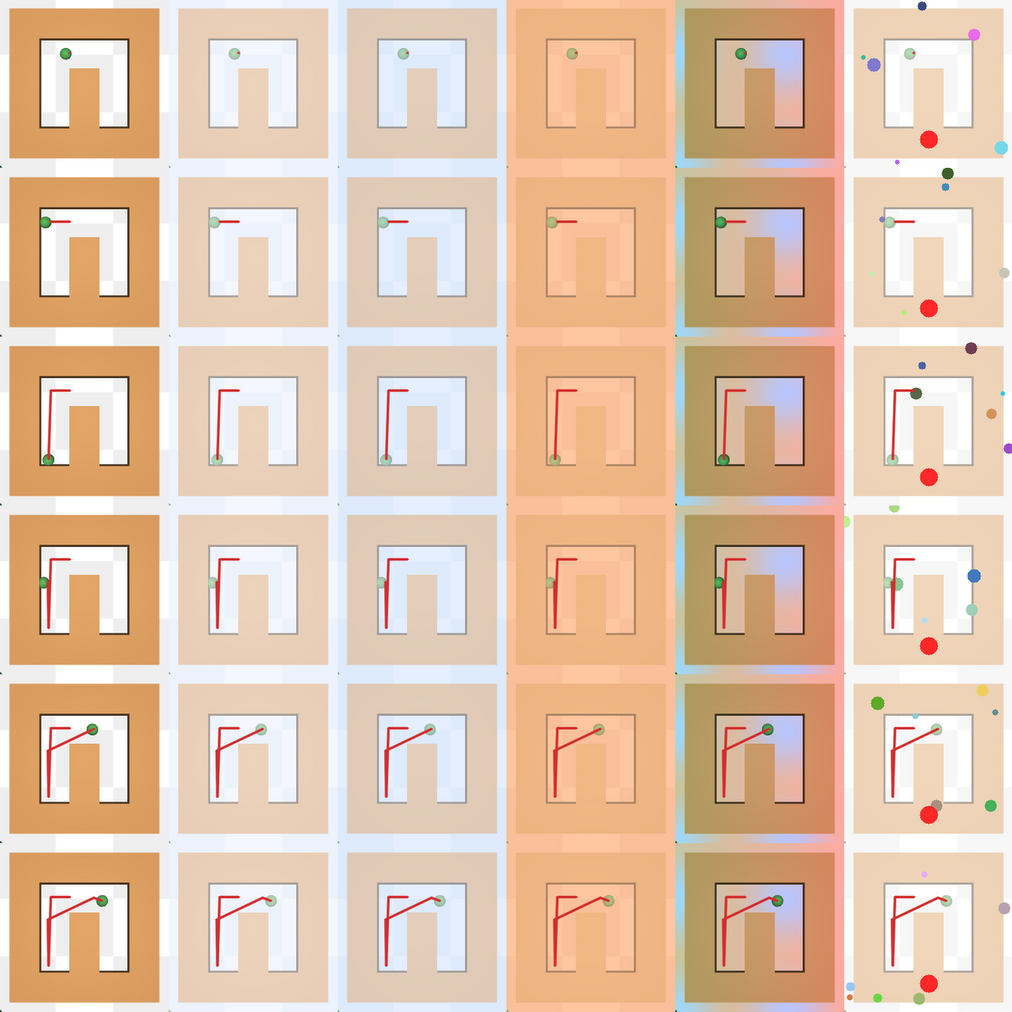
\includegraphics[width=\textwidth]{docs/figures/rollout_examples/pointmaze_dinowm_unsuccessful_iclr.pdf}
    \caption{PointMaze, DINO-WM (unsuccessful).}
    \label{fig:rollout-pm-wm-fail}
  \end{subfigure}\\[0.6em]
  \begin{subfigure}[t]{\textwidth}
    \centering
    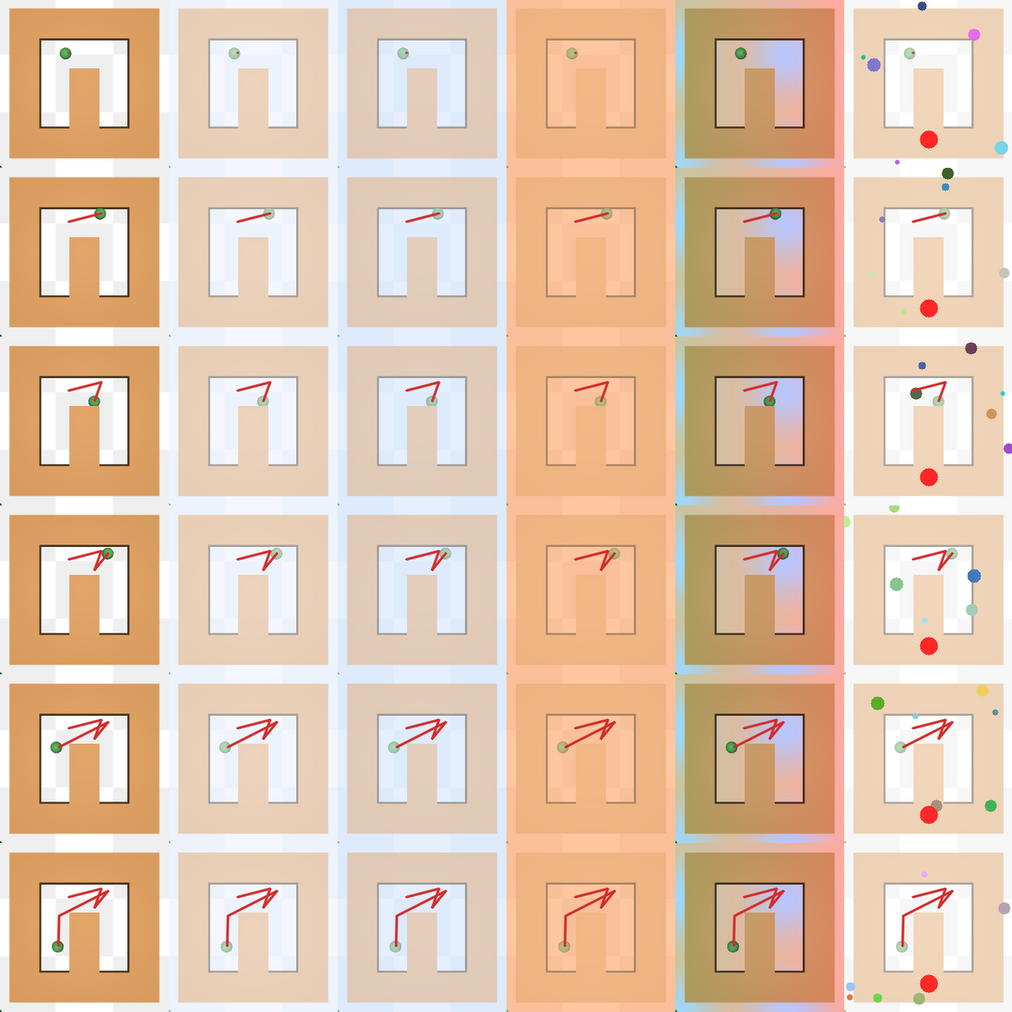
\includegraphics[width=\textwidth]{docs/figures/rollout_examples/pointmaze_dinobisim_successful_iclr.pdf}
    \caption{PointMaze, DINO-Bisim (successful).}
    \label{fig:rollout-pm-bisim-succ}
  \end{subfigure}\\[0.6em]
  \begin{subfigure}[t]{\textwidth}
    \centering
    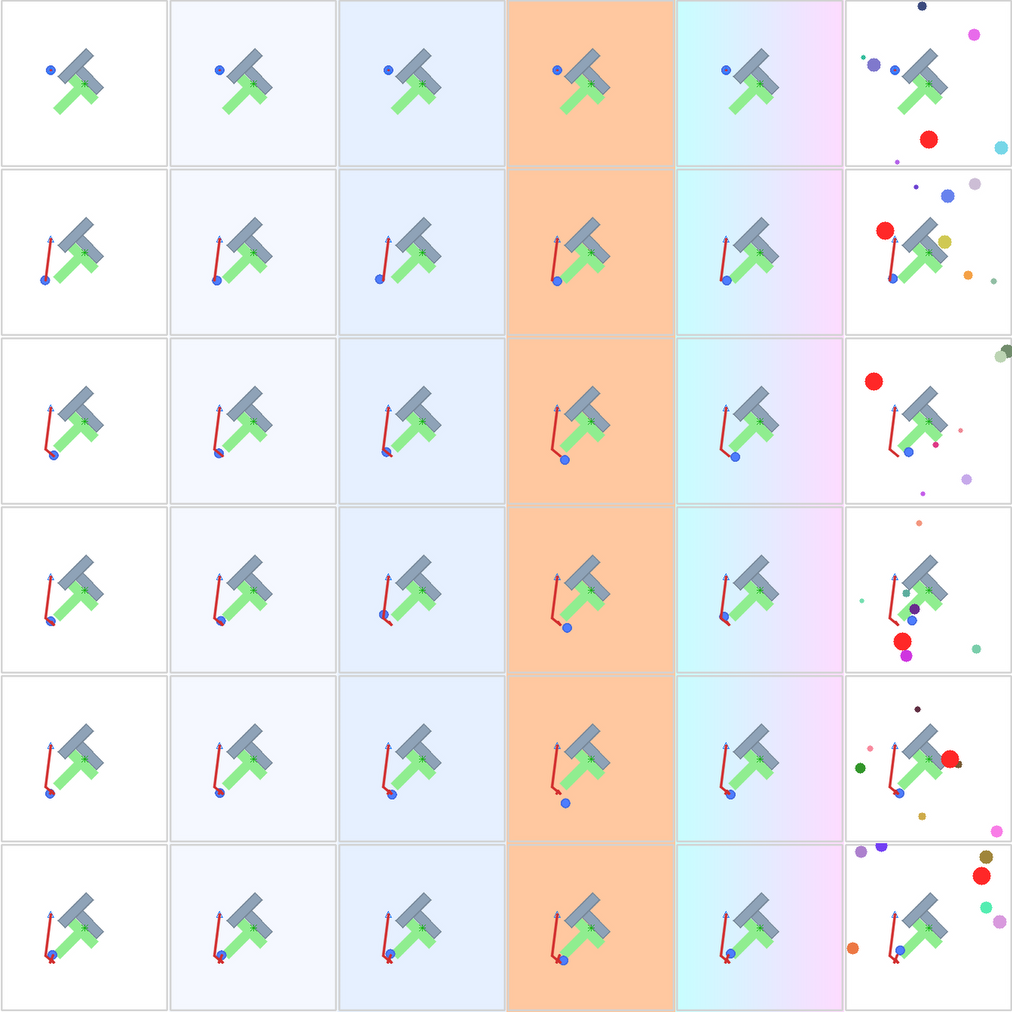
\includegraphics[width=\textwidth]{docs/figures/rollout_examples/pusht_dinowm_unsuccessful_iclr.pdf}
    \caption{PushT, DINO-WM (unsuccessful).}
    \label{fig:rollout-pt-wm-fail}
  \end{subfigure}\\[0.6em]
  \begin{subfigure}[t]{\textwidth}
    \centering
    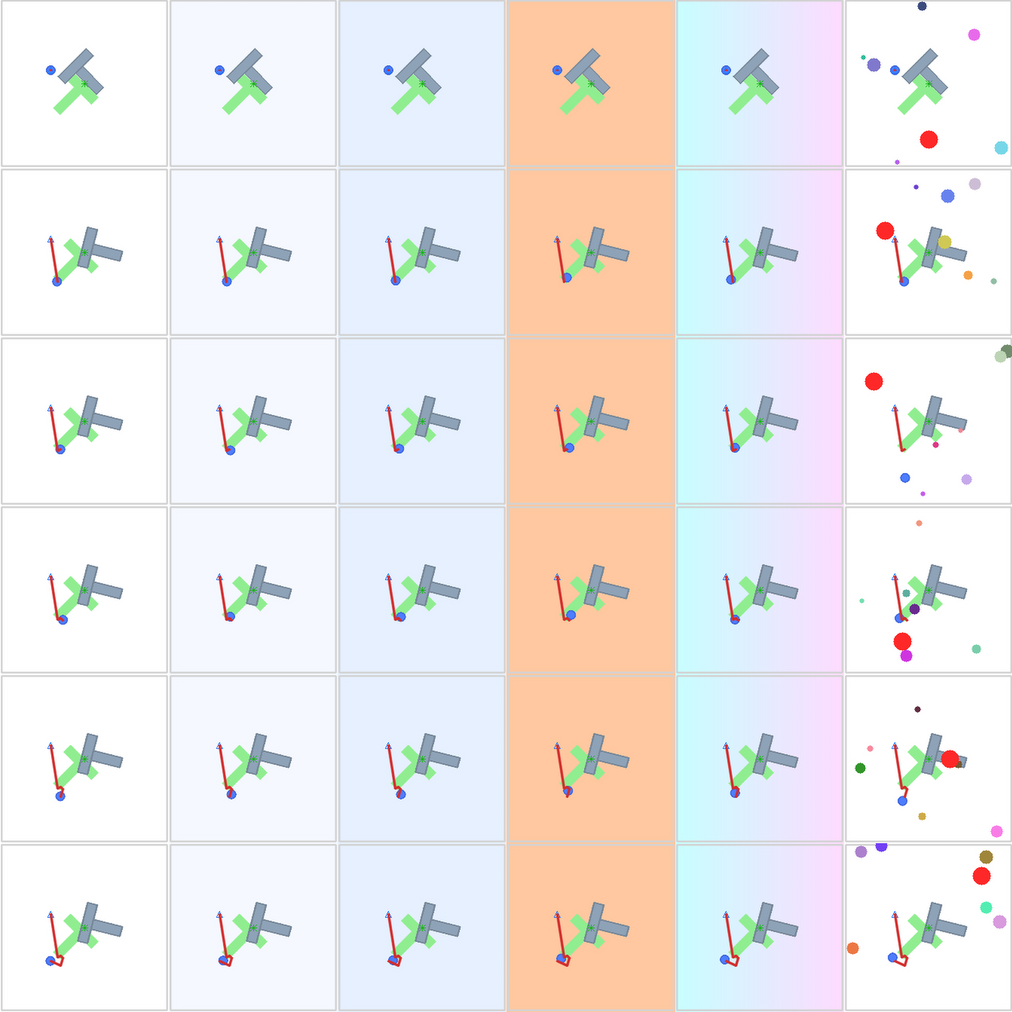
\includegraphics[width=\textwidth]{docs/figures/rollout_examples/pusht_dinobisim_successful_iclr.pdf}
    \caption{PushT, DINO-Bisim (successful).}
    \label{fig:rollout-pt-bisim-succ}
  \end{subfigure}
  \caption{%
    \textbf{Visual planning rollouts under test-time appearance shift.}
    Each panel is a $6{\times}6$ grid: \emph{rows} are MPC replanning steps ($t{=}1,\ldots,6$); \emph{columns} are the six lighting/color test conditions NC, SC, C, LC, LCG, and~D (dynamic distractors).
    Orange marker: start state; green marker: goal.
    Red polyline: executed trajectory from start through the current step.
    PointMaze uses the U-maze simulator; PushT uses the block-pushing contact task.
    Within each task, the unsuccessful (DINO-WM) and successful (DINO-Bisim) examples share the same initial state and goal; only the planned actions differ.
    DINO-WM often drifts or stalls under large background shifts (e.g., LC, LCG), whereas DINO-Bisim reaches the goal more reliably across conditions.
  }
  \label{fig:rollout-examples}
\end{figure*}

% ---------------------------------------------------------------------------
% Option B — standalone captions (one figure per PDF)
% ---------------------------------------------------------------------------

% --- PointMaze, DINO-WM, failure ---
% \begin{figure}[t]
%   \centering
%   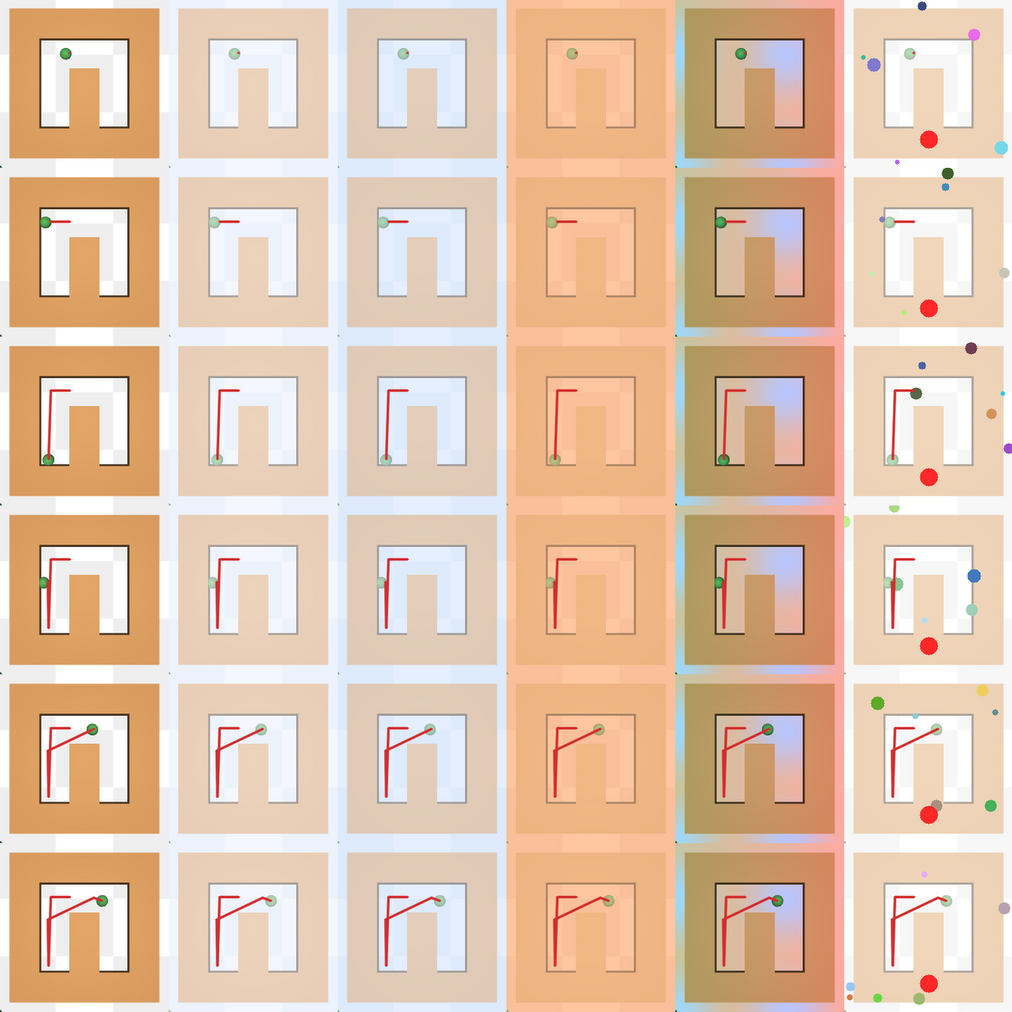
\includegraphics[width=\textwidth]{docs/figures/rollout_examples/pointmaze_dinowm_unsuccessful_iclr.pdf}
%   \caption{%
%     \textbf{PointMaze planning failure (DINO-WM).}
%     Six MPC steps (rows) under six visual conditions (columns: NC, SC, C, LC, LCG, D).
%     Markers: start (orange), goal (green); red line: rollout path.
%     Same init/goal as Fig.~\ref{fig:rollout-pm-bisim-succ}; WM fails to reach the goal, especially under LC/LCG.
%   }
%   \label{fig:rollout-pm-wm-fail}
% \end{figure}

% --- PointMaze, DINO-Bisim, success ---
% \begin{figure}[t]
%   \centering
%   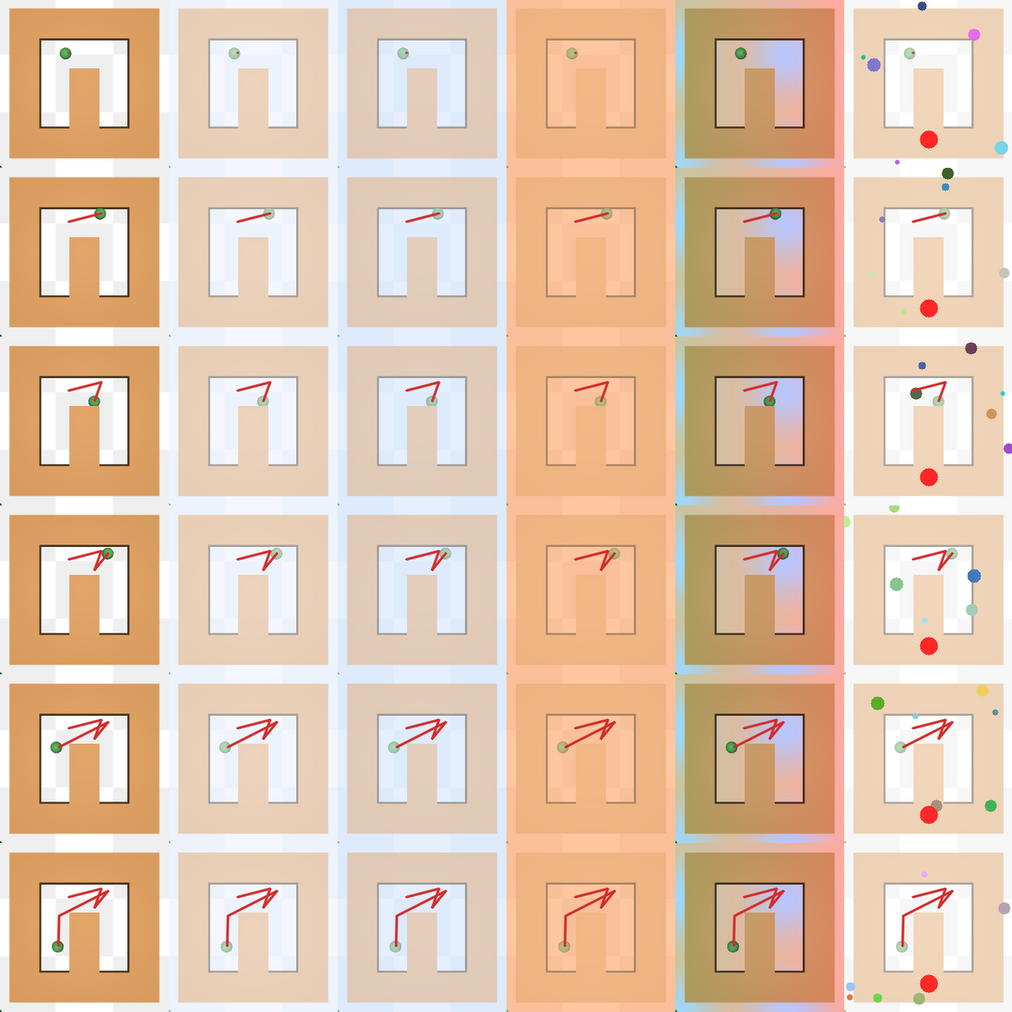
\includegraphics[width=\textwidth]{docs/figures/rollout_examples/pointmaze_dinobisim_successful_iclr.pdf}
%   \caption{%
%     \textbf{PointMaze planning success (DINO-Bisim).}
%     Same layout and shared episode as Fig.~\ref{fig:rollout-pm-wm-fail}.
%     Bisimulation-aligned representations yield a goal-reaching trajectory across all six appearance conditions.
%   }
%   \label{fig:rollout-pm-bisim-succ}
% \end{figure}

% --- PushT, DINO-WM, failure ---
% \begin{figure}[t]
%   \centering
%   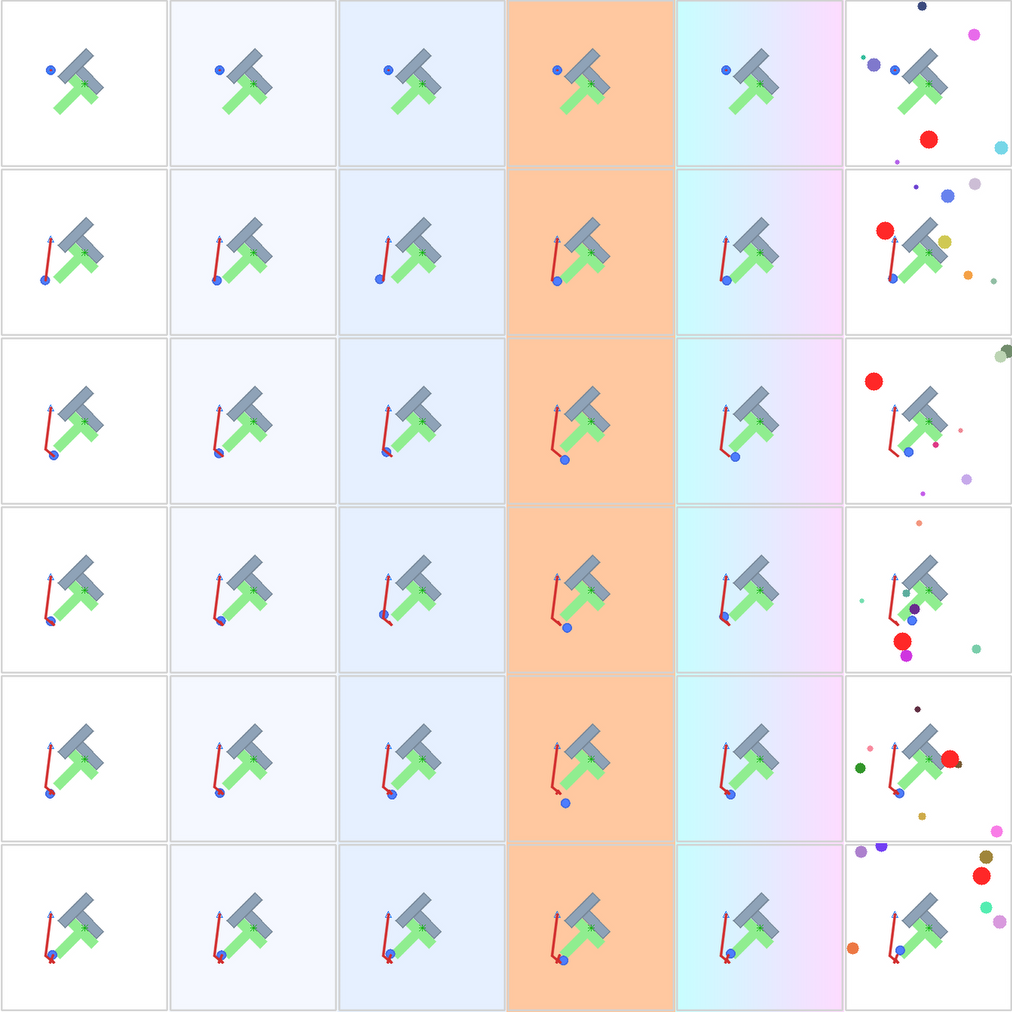
\includegraphics[width=\textwidth]{docs/figures/rollout_examples/pusht_dinowm_unsuccessful_iclr.pdf}
%   \caption{%
%     \textbf{PushT planning failure (DINO-WM).}
%     Six MPC steps $\times$ six visual conditions; start/goal markers and executed path overlaid.
%     Matched init/goal with Fig.~\ref{fig:rollout-pt-bisim-succ}.
%     WM misaligns the block with the target pose under shifted backgrounds.
%   }
%   \label{fig:rollout-pt-wm-fail}
% \end{figure}

% --- PushT, DINO-Bisim, success ---
% \begin{figure}[t]
%   \centering
%   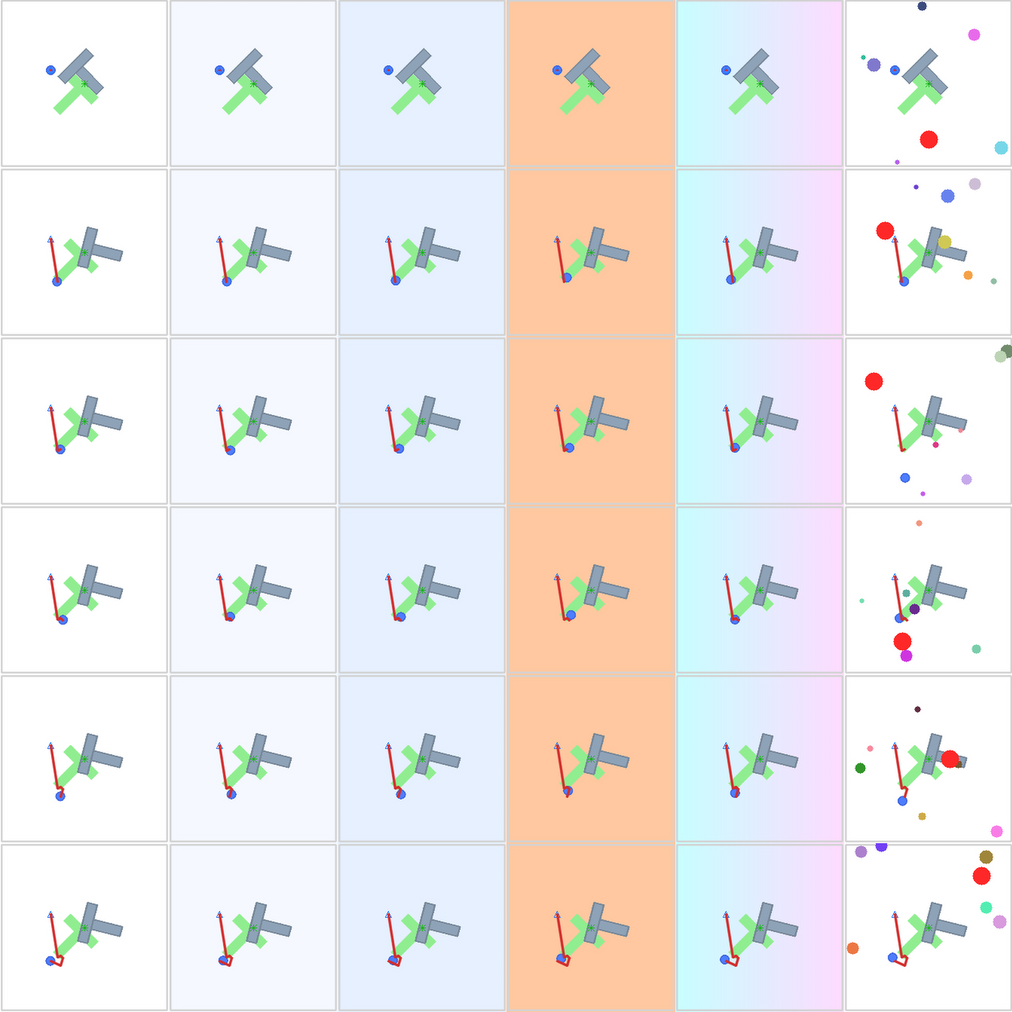
\includegraphics[width=\textwidth]{docs/figures/rollout_examples/pusht_dinobisim_successful_iclr.pdf}
%   \caption{%
%     \textbf{PushT planning success (DINO-Bisim).}
%     Same episode as Fig.~\ref{fig:rollout-pt-wm-fail}.
%     DINO-Bisim completes the push despite lighting/color perturbations at test time.
%   }
%   \label{fig:rollout-pt-bisim-succ}
% \end{figure}

% ---------------------------------------------------------------------------
% Short inline text (for main paper, ~2 sentences)
% ---------------------------------------------------------------------------
% Fig.~\ref{fig:rollout-examples} shows representative MPC rollouts on PointMaze and PushT
% under six test-time visual conditions (columns) over six replanning steps (rows).
% DINO-WM (top/bottom-left pairs) fails under strong appearance shift while DINO-Bisim
% (paired success rows) reaches the goal from the same start and target.
